\documentclass[a4paper,11pt]{article}

\usepackage[italian]{babel}

\usepackage[latin1]{inputenc}

\usepackage[T1]{fontenc}

\usepackage{graphicx}

\usepackage{indentfirst}

\usepackage{amsmath,amssymb}

\usepackage{enumitem} 

\newcommand{\virgolette}[1]{``#1''}

\usepackage[margin=1in]{geometry} %Smaller margins

\usepackage{lmodern} %Vector PDF

\usepackage{siunitx}

\usepackage{xcolor}

\usepackage{colortbl}

\usepackage{multirow}

\usepackage{rotating}

\usepackage{booktabs}

\usepackage{longtable}

\usepackage{graphicx}
\graphicspath{ {Images/} }

\usepackage{wrapfig}

\begin{document}

	\section{Introduzione}
		
		Obbiettivo finale di questo esperimento � quello di determinare il coefficiente di correlazione $n$ del vetro di cui � composto un prism, o, pi� propriamente di verificare la legge di dispersione secondo la legge di Cauchy qui di seguito

	\begin{equation}\label{Cauchy}
		n^2(\lambda)=a+\frac{b}{\lambda^2}.
	\end{equation}
	
	\begin{figure}[h]
		\centering
    	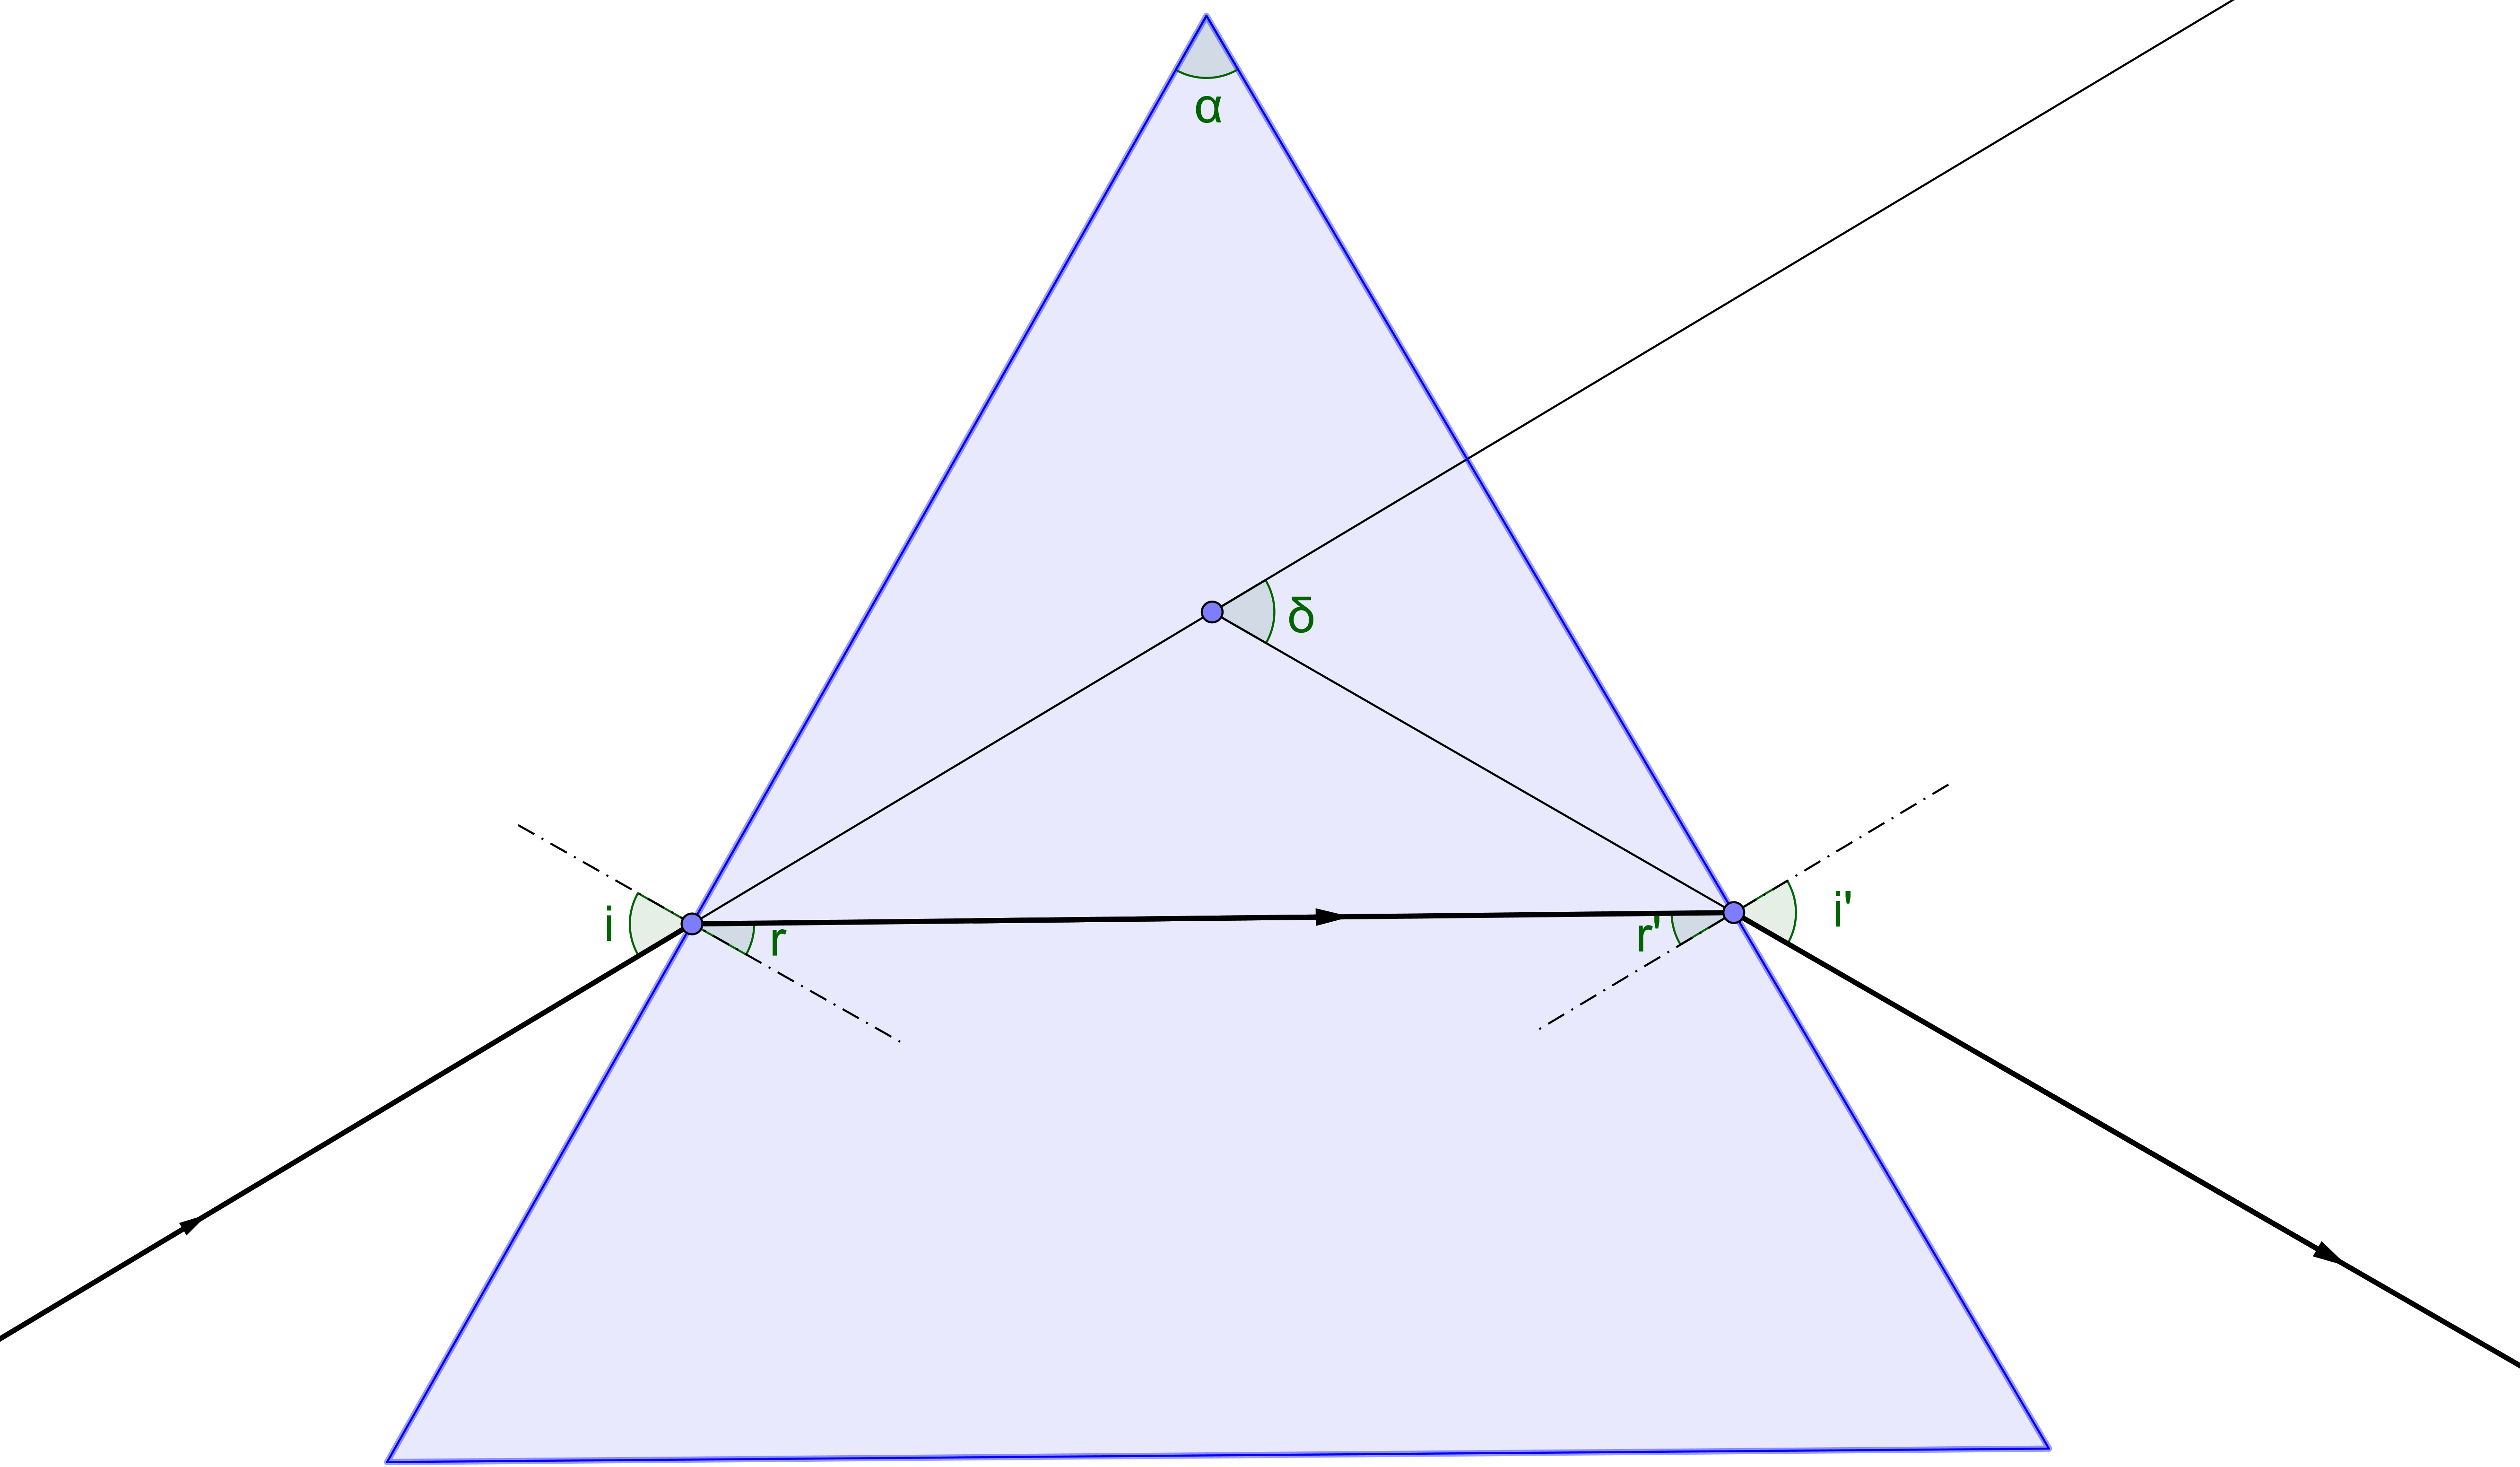
\includegraphics[width=1\textwidth]{Prisma}
    	\caption{Schema della sezione del prisma}	
	\end{figure}	
	
	Tuttavia prima di arrivare a questo punto sar� necessario adempire a tappe intermedie quali la misurazione dell'angolo $\alpha$ caratterizzante il prisma e, subito dopo la ricerca dell'angolo di deviazione minima per ogni colore dello spettro della lampada di Hg. Lo spettro del mercurio era stato trovato e analizzato nell'esperienza precedente. Denotando con $i$ l'angolo di incidenza e con $i'$ l'angolo di emergenza, con $r$ l'angolo in uscita dalla prima faccia, con $r'$ l'angolo in entrata nella seconda faccia e con $\delta$ l'angolo di deviazione, si scrivono le seguenti relazioni:
	
	\begin{equation}
		r+r'=\alpha \qquad \delta = i+i'-\alpha
	\end{equation}
	
	e
	
	\begin{equation}
		\frac{\sin i}{\sin r} = n \qquad \frac{\sin r'}{\sin i} = \frac{1}{n}.
	\end{equation}	
	
	Cercando il minimo della funzione $\delta = \delta (i)$ per derivazione, con un po' di algebra si arriva alla condizione
	
	\begin{equation}
		i = i' \qquad r = r'
	\end{equation}
	
	ossia il raggio di luce deve essere ortogonale alla bisettrice del prisma. Attraverso le \ref{Cauchy}, si ricava
	
	\begin{equation}
		\delta_m = 2i_m - \alpha \qquad r_m = \frac{\alpha}{2} \qquad \sin i_m = n\sin \left( \frac{\alpha}{2} \right)
	\end{equation}
	
	Da cui si pu� ottenere la formula definitiva per $n$
	
	\begin{equation} \label{n}
		n(\lambda) = \frac{\sin \frac{\alpha+\delta _m}{2}}{\sin \frac{\alpha}{2}}.
	\end{equation}
	
	Si andr� quindi a misurare l'angolo $\alpha$ di un prisma e l'angolo $\delta _m$ per diverse lunghezze d'onda della lampada di mercurio, che presenta uno spettro ben visibile e ben distribuito su tutto lo spettro visibile. Dall'analisi di questi dati sar� possibile ricavare la legge di Cauchy, come mostreremo successivamente.

\end{document}
